\documentclass[twoside]{book}

% Packages required by doxygen
\usepackage{fixltx2e}
\usepackage{calc}
\usepackage{doxygen}
\usepackage[export]{adjustbox} % also loads graphicx
\usepackage{graphicx}
\usepackage[utf8]{inputenc}
\usepackage{makeidx}
\usepackage{multicol}
\usepackage{multirow}
\PassOptionsToPackage{warn}{textcomp}
\usepackage{textcomp}
\usepackage[nointegrals]{wasysym}
\usepackage[table]{xcolor}

% Font selection
\usepackage[T1]{fontenc}
\usepackage[scaled=.90]{helvet}
\usepackage{courier}
\usepackage{amssymb}
\usepackage{sectsty}
\renewcommand{\familydefault}{\sfdefault}
\allsectionsfont{%
  \fontseries{bc}\selectfont%
  \color{darkgray}%
}
\renewcommand{\DoxyLabelFont}{%
  \fontseries{bc}\selectfont%
  \color{darkgray}%
}
\newcommand{\+}{\discretionary{\mbox{\scriptsize$\hookleftarrow$}}{}{}}

% Page & text layout
\usepackage{geometry}
\geometry{%
  a4paper,%
  top=2.5cm,%
  bottom=2.5cm,%
  left=2.5cm,%
  right=2.5cm%
}
\tolerance=750
\hfuzz=15pt
\hbadness=750
\setlength{\emergencystretch}{15pt}
\setlength{\parindent}{0cm}
\setlength{\parskip}{0.2cm}
\makeatletter
\renewcommand{\paragraph}{%
  \@startsection{paragraph}{4}{0ex}{-1.0ex}{1.0ex}{%
    \normalfont\normalsize\bfseries\SS@parafont%
  }%
}
\renewcommand{\subparagraph}{%
  \@startsection{subparagraph}{5}{0ex}{-1.0ex}{1.0ex}{%
    \normalfont\normalsize\bfseries\SS@subparafont%
  }%
}
\makeatother

% Headers & footers
\usepackage{fancyhdr}
\pagestyle{fancyplain}
\fancyhead[LE]{\fancyplain{}{\bfseries\thepage}}
\fancyhead[CE]{\fancyplain{}{}}
\fancyhead[RE]{\fancyplain{}{\bfseries\leftmark}}
\fancyhead[LO]{\fancyplain{}{\bfseries\rightmark}}
\fancyhead[CO]{\fancyplain{}{}}
\fancyhead[RO]{\fancyplain{}{\bfseries\thepage}}
\fancyfoot[LE]{\fancyplain{}{}}
\fancyfoot[CE]{\fancyplain{}{}}
\fancyfoot[RE]{\fancyplain{}{\bfseries\scriptsize Generated on Thu Dec 15 2016 14\+:05\+:50 for My Project by Doxygen }}
\fancyfoot[LO]{\fancyplain{}{\bfseries\scriptsize Generated on Thu Dec 15 2016 14\+:05\+:50 for My Project by Doxygen }}
\fancyfoot[CO]{\fancyplain{}{}}
\fancyfoot[RO]{\fancyplain{}{}}
\renewcommand{\footrulewidth}{0.4pt}
\renewcommand{\chaptermark}[1]{%
  \markboth{#1}{}%
}
\renewcommand{\sectionmark}[1]{%
  \markright{\thesection\ #1}%
}

% Indices & bibliography
\usepackage{natbib}
\usepackage[titles]{tocloft}
\setcounter{tocdepth}{3}
\setcounter{secnumdepth}{5}
\makeindex

% Hyperlinks (required, but should be loaded last)
\usepackage{ifpdf}
\ifpdf
  \usepackage[pdftex,pagebackref=true]{hyperref}
\else
  \usepackage[ps2pdf,pagebackref=true]{hyperref}
\fi
\hypersetup{%
  colorlinks=true,%
  linkcolor=blue,%
  citecolor=blue,%
  unicode%
}

% Custom commands
\newcommand{\clearemptydoublepage}{%
  \newpage{\pagestyle{empty}\cleardoublepage}%
}


%===== C O N T E N T S =====

\begin{document}

% Titlepage & ToC
\hypersetup{pageanchor=false,
             bookmarks=true,
             bookmarksnumbered=true,
             pdfencoding=unicode
            }
\pagenumbering{roman}
\begin{titlepage}
\vspace*{7cm}
\begin{center}%
{\Large My Project }\\
\vspace*{1cm}
{\large Generated by Doxygen 1.8.10}\\
\vspace*{0.5cm}
{\small Thu Dec 15 2016 14:05:50}\\
\end{center}
\end{titlepage}
\clearemptydoublepage
\tableofcontents
\clearemptydoublepage
\pagenumbering{arabic}
\hypersetup{pageanchor=true}

%--- Begin generated contents ---
\chapter{quiz}
\label{md__r_e_a_d_m_e}
\hypertarget{md__r_e_a_d_m_e}{}
software Design and Quality \hyperlink{class_quiz}{Quiz}

Simple quiz for the above topic written in c++ 
\chapter{Hierarchical Index}
\section{Class Hierarchy}
This inheritance list is sorted roughly, but not completely, alphabetically\+:\begin{DoxyCompactList}
\item \contentsline{section}{Quiz}{\pageref{class_quiz}}{}
\item \contentsline{section}{User}{\pageref{class_user}}{}
\begin{DoxyCompactList}
\item \contentsline{section}{Admin}{\pageref{class_admin}}{}
\item \contentsline{section}{Admin}{\pageref{class_admin}}{}
\item \contentsline{section}{Student}{\pageref{class_student}}{}
\item \contentsline{section}{Student}{\pageref{class_student}}{}
\end{DoxyCompactList}
\end{DoxyCompactList}

\chapter{Class Index}
\section{Class List}
Here are the classes, structs, unions and interfaces with brief descriptions\+:\begin{DoxyCompactList}
\item\contentsline{section}{\hyperlink{class_admin}{Admin} }{\pageref{class_admin}}{}
\item\contentsline{section}{\hyperlink{structtinyxml2_1_1_entity}{tinyxml2\+::\+Entity} }{\pageref{structtinyxml2_1_1_entity}}{}
\item\contentsline{section}{\hyperlink{structtinyxml2_1_1_long_fits_into_size_t_minus_one}{tinyxml2\+::\+Long\+Fits\+Into\+Size\+T\+Minus\+One$<$ bool $>$} }{\pageref{structtinyxml2_1_1_long_fits_into_size_t_minus_one}}{}
\item\contentsline{section}{\hyperlink{structtinyxml2_1_1_long_fits_into_size_t_minus_one_3_01false_01_4}{tinyxml2\+::\+Long\+Fits\+Into\+Size\+T\+Minus\+One$<$ false $>$} }{\pageref{structtinyxml2_1_1_long_fits_into_size_t_minus_one_3_01false_01_4}}{}
\item\contentsline{section}{\hyperlink{class_quiz}{Quiz} }{\pageref{class_quiz}}{}
\item\contentsline{section}{\hyperlink{class_student}{Student} }{\pageref{class_student}}{}
\item\contentsline{section}{\hyperlink{class_user}{User} }{\pageref{class_user}}{}
\end{DoxyCompactList}

\chapter{Class Documentation}
\hypertarget{class_admin}{}\section{Admin Class Reference}
\label{class_admin}\index{Admin@{Admin}}


{\ttfamily \#include $<$quiz.\+h$>$}

Inheritance diagram for Admin\+:\begin{figure}[H]
\begin{center}
\leavevmode
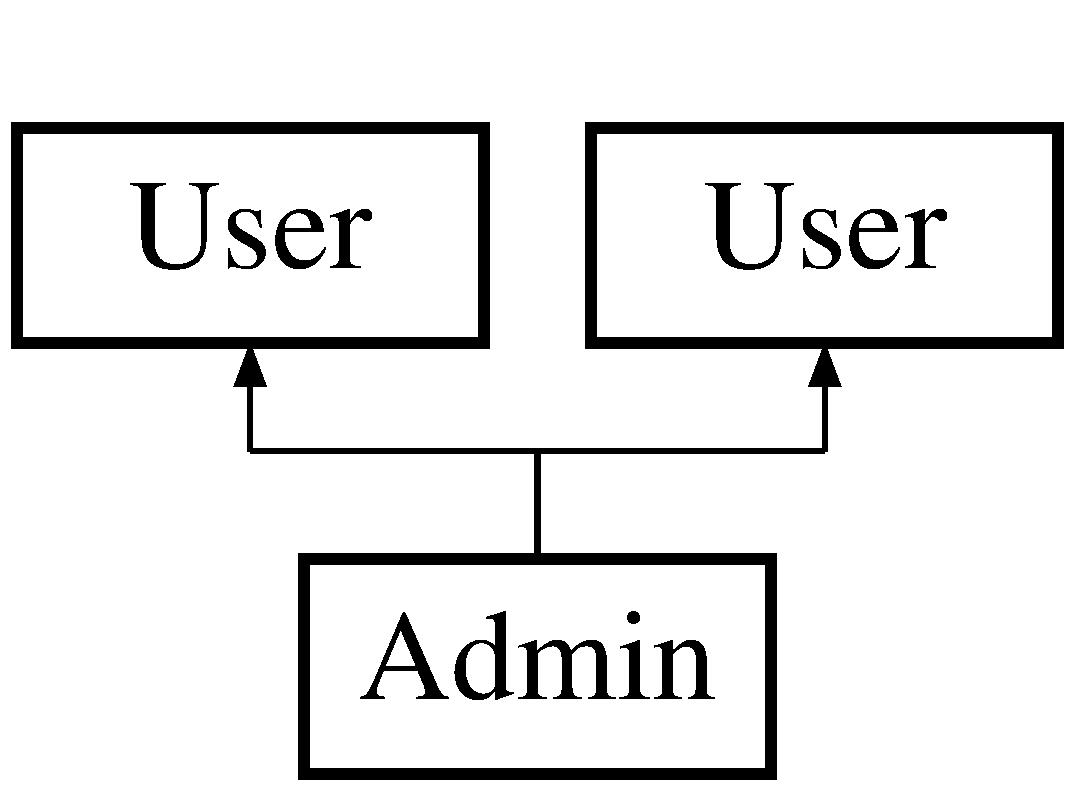
\includegraphics[height=2.000000cm]{class_admin}
\end{center}
\end{figure}
\subsection*{Public Member Functions}
\begin{DoxyCompactItemize}
\item 
void \hyperlink{class_admin_a3064fddba449b5699678dae6218fc3b8}{view} (int \hyperlink{class_user_aa7e6e39b43020bbe9c3a196b3689b0f7}{id}, string \hyperlink{class_user_a643f85779a4693855c171c396f49e515}{name})
\item 
void \hyperlink{class_admin_a7ff3c33183ba1b6dee66c5e8b1aac386}{remove} ()
\item 
void \hyperlink{class_admin_a7d8d62a090555b8ee72e3a3c78f32036}{add} ()
\item 
void \hyperlink{class_admin_a3064fddba449b5699678dae6218fc3b8}{view} (int \hyperlink{class_user_aa7e6e39b43020bbe9c3a196b3689b0f7}{id}, string \hyperlink{class_user_a643f85779a4693855c171c396f49e515}{name})
\item 
void \hyperlink{class_admin_a7ff3c33183ba1b6dee66c5e8b1aac386}{remove} ()
\item 
void \hyperlink{class_admin_a7d8d62a090555b8ee72e3a3c78f32036}{add} ()
\end{DoxyCompactItemize}
\subsection*{Additional Inherited Members}


\subsection{Detailed Description}
\hyperlink{class_admin}{Admin} class inherited from \hyperlink{class_user}{User} class 

\subsection{Member Function Documentation}
\hypertarget{class_admin_a7d8d62a090555b8ee72e3a3c78f32036}{}\index{Admin@{Admin}!add@{add}}
\index{add@{add}!Admin@{Admin}}
\subsubsection[{add()}]{\setlength{\rightskip}{0pt plus 5cm}void Admin\+::add (
\begin{DoxyParamCaption}
{}
\end{DoxyParamCaption}
)}\label{class_admin_a7d8d62a090555b8ee72e3a3c78f32036}
function to add a question from question databank \hypertarget{class_admin_a7d8d62a090555b8ee72e3a3c78f32036}{}\index{Admin@{Admin}!add@{add}}
\index{add@{add}!Admin@{Admin}}
\subsubsection[{add()}]{\setlength{\rightskip}{0pt plus 5cm}void Admin\+::add (
\begin{DoxyParamCaption}
{}
\end{DoxyParamCaption}
)}\label{class_admin_a7d8d62a090555b8ee72e3a3c78f32036}
function to add a question from question databank \hypertarget{class_admin_a7ff3c33183ba1b6dee66c5e8b1aac386}{}\index{Admin@{Admin}!remove@{remove}}
\index{remove@{remove}!Admin@{Admin}}
\subsubsection[{remove()}]{\setlength{\rightskip}{0pt plus 5cm}void Admin\+::remove (
\begin{DoxyParamCaption}
{}
\end{DoxyParamCaption}
)}\label{class_admin_a7ff3c33183ba1b6dee66c5e8b1aac386}
function to remove a question from question databank \hypertarget{class_admin_a7ff3c33183ba1b6dee66c5e8b1aac386}{}\index{Admin@{Admin}!remove@{remove}}
\index{remove@{remove}!Admin@{Admin}}
\subsubsection[{remove()}]{\setlength{\rightskip}{0pt plus 5cm}void Admin\+::remove (
\begin{DoxyParamCaption}
{}
\end{DoxyParamCaption}
)}\label{class_admin_a7ff3c33183ba1b6dee66c5e8b1aac386}
function to remove a question from question databank \hypertarget{class_admin_a3064fddba449b5699678dae6218fc3b8}{}\index{Admin@{Admin}!view@{view}}
\index{view@{view}!Admin@{Admin}}
\subsubsection[{view(int id, string name)}]{\setlength{\rightskip}{0pt plus 5cm}void Admin\+::view (
\begin{DoxyParamCaption}
\item[{int}]{id, }
\item[{string}]{name}
\end{DoxyParamCaption}
)}\label{class_admin_a3064fddba449b5699678dae6218fc3b8}
function to retrieve and display student profile \hypertarget{class_admin_a3064fddba449b5699678dae6218fc3b8}{}\index{Admin@{Admin}!view@{view}}
\index{view@{view}!Admin@{Admin}}
\subsubsection[{view(int id, string name)}]{\setlength{\rightskip}{0pt plus 5cm}void Admin\+::view (
\begin{DoxyParamCaption}
\item[{int}]{id, }
\item[{string}]{name}
\end{DoxyParamCaption}
)}\label{class_admin_a3064fddba449b5699678dae6218fc3b8}
function to retrieve and display student profile 

The documentation for this class was generated from the following files\+:\begin{DoxyCompactItemize}
\item 
main.\+cpp\item 
quiz.\+h\end{DoxyCompactItemize}

\hypertarget{structtinyxml2_1_1_entity}{}\section{tinyxml2\+:\+:Entity Struct Reference}
\label{structtinyxml2_1_1_entity}\index{tinyxml2\+::\+Entity@{tinyxml2\+::\+Entity}}
\subsection*{Public Attributes}
\begin{DoxyCompactItemize}
\item 
\hypertarget{structtinyxml2_1_1_entity_ab330f5d665d29bfc811ecfa76315894b}{}const char $\ast$ {\bfseries pattern}\label{structtinyxml2_1_1_entity_ab330f5d665d29bfc811ecfa76315894b}

\item 
\hypertarget{structtinyxml2_1_1_entity_a25e2b57cb59cb4fa68f283d7cb570f21}{}int {\bfseries length}\label{structtinyxml2_1_1_entity_a25e2b57cb59cb4fa68f283d7cb570f21}

\item 
\hypertarget{structtinyxml2_1_1_entity_a7334e81e33b4615655a403711b24f3ed}{}char {\bfseries value}\label{structtinyxml2_1_1_entity_a7334e81e33b4615655a403711b24f3ed}

\end{DoxyCompactItemize}


The documentation for this struct was generated from the following file\+:\begin{DoxyCompactItemize}
\item 
tinyxml2.\+cpp\end{DoxyCompactItemize}

\hypertarget{structtinyxml2_1_1_long_fits_into_size_t_minus_one}{}\section{tinyxml2\+:\+:Long\+Fits\+Into\+Size\+T\+Minus\+One$<$ bool $>$ Struct Template Reference}
\label{structtinyxml2_1_1_long_fits_into_size_t_minus_one}\index{tinyxml2\+::\+Long\+Fits\+Into\+Size\+T\+Minus\+One$<$ bool $>$@{tinyxml2\+::\+Long\+Fits\+Into\+Size\+T\+Minus\+One$<$ bool $>$}}
\subsection*{Static Public Member Functions}
\begin{DoxyCompactItemize}
\item 
\hypertarget{structtinyxml2_1_1_long_fits_into_size_t_minus_one_a3057710104ab733963eb32fda0bc374c}{}static bool {\bfseries Fits} (unsigned long value)\label{structtinyxml2_1_1_long_fits_into_size_t_minus_one_a3057710104ab733963eb32fda0bc374c}

\end{DoxyCompactItemize}


The documentation for this struct was generated from the following file\+:\begin{DoxyCompactItemize}
\item 
tinyxml2.\+cpp\end{DoxyCompactItemize}

\hypertarget{structtinyxml2_1_1_long_fits_into_size_t_minus_one_3_01false_01_4}{}\section{tinyxml2\+:\+:Long\+Fits\+Into\+Size\+T\+Minus\+One$<$ false $>$ Struct Template Reference}
\label{structtinyxml2_1_1_long_fits_into_size_t_minus_one_3_01false_01_4}\index{tinyxml2\+::\+Long\+Fits\+Into\+Size\+T\+Minus\+One$<$ false $>$@{tinyxml2\+::\+Long\+Fits\+Into\+Size\+T\+Minus\+One$<$ false $>$}}
\subsection*{Static Public Member Functions}
\begin{DoxyCompactItemize}
\item 
\hypertarget{structtinyxml2_1_1_long_fits_into_size_t_minus_one_3_01false_01_4_a29b01087f38a951276df69d358dc0764}{}static bool {\bfseries Fits} (unsigned long)\label{structtinyxml2_1_1_long_fits_into_size_t_minus_one_3_01false_01_4_a29b01087f38a951276df69d358dc0764}

\end{DoxyCompactItemize}


The documentation for this struct was generated from the following file\+:\begin{DoxyCompactItemize}
\item 
tinyxml2.\+cpp\end{DoxyCompactItemize}

\hypertarget{class_quiz}{}\section{Quiz Class Reference}
\label{class_quiz}\index{Quiz@{Quiz}}
\subsection*{Public Member Functions}
\begin{DoxyCompactItemize}
\item 
\hypertarget{class_quiz_a585d5f112cbf72932fff7983c1e5b2c9}{}void {\bfseries read} ()\label{class_quiz_a585d5f112cbf72932fff7983c1e5b2c9}

\item 
void \hyperlink{class_quiz_a318cf3e77db0c2a994752ef0541792bf}{make\+Qs} (string $\ast$\hyperlink{class_quiz_a8d26a1bec061915e1095808386fa64f6}{question}, int $\ast$answer)
\item 
void \hyperlink{class_quiz_a31824f4cb143442fb30d05d5193e6e90}{send\+Q} (string $\ast$\hyperlink{class_quiz_a8d26a1bec061915e1095808386fa64f6}{question})
\item 
bool \hyperlink{class_quiz_a04872049618df0469f083b226f68eb16}{verify\+Qs} (char answer)
\item 
void \hyperlink{class_quiz_aefcae0c2187864f7764e3a2cc536f723}{report} (int id, string profile\+\_\+type)
\item 
void \hyperlink{class_quiz_a2a30f1d27f8a873dedbf4a19c4143f31}{save} ()
\end{DoxyCompactItemize}
\subsection*{Public Attributes}
\begin{DoxyCompactItemize}
\item 
string \hyperlink{class_quiz_a8d26a1bec061915e1095808386fa64f6}{question} \mbox{[}$\,$\mbox{]}
\item 
int \hyperlink{class_quiz_a19d4b1d98b6ae6cebda04923b37e2aaf}{answers} \mbox{[}$\,$\mbox{]}
\end{DoxyCompactItemize}


\subsection{Detailed Description}
\hyperlink{class_quiz}{Quiz} class 

\subsection{Member Function Documentation}
\hypertarget{class_quiz_a318cf3e77db0c2a994752ef0541792bf}{}\index{Quiz@{Quiz}!make\+Qs@{make\+Qs}}
\index{make\+Qs@{make\+Qs}!Quiz@{Quiz}}
\subsubsection[{make\+Qs(string $\ast$question, int $\ast$answer)}]{\setlength{\rightskip}{0pt plus 5cm}void Quiz\+::make\+Qs (
\begin{DoxyParamCaption}
\item[{string $\ast$}]{question, }
\item[{int $\ast$}]{answer}
\end{DoxyParamCaption}
)}\label{class_quiz_a318cf3e77db0c2a994752ef0541792bf}
Function to fetch 10 random questions from database \hypertarget{class_quiz_aefcae0c2187864f7764e3a2cc536f723}{}\index{Quiz@{Quiz}!report@{report}}
\index{report@{report}!Quiz@{Quiz}}
\subsubsection[{report(int id, string profile\+\_\+type)}]{\setlength{\rightskip}{0pt plus 5cm}void Quiz\+::report (
\begin{DoxyParamCaption}
\item[{int}]{id, }
\item[{string}]{profile\+\_\+type}
\end{DoxyParamCaption}
)}\label{class_quiz_aefcae0c2187864f7764e3a2cc536f723}
generate and print report \hypertarget{class_quiz_a2a30f1d27f8a873dedbf4a19c4143f31}{}\index{Quiz@{Quiz}!save@{save}}
\index{save@{save}!Quiz@{Quiz}}
\subsubsection[{save()}]{\setlength{\rightskip}{0pt plus 5cm}void Quiz\+::save (
\begin{DoxyParamCaption}
{}
\end{DoxyParamCaption}
)}\label{class_quiz_a2a30f1d27f8a873dedbf4a19c4143f31}
save quiz result \& report \hypertarget{class_quiz_a31824f4cb143442fb30d05d5193e6e90}{}\index{Quiz@{Quiz}!send\+Q@{send\+Q}}
\index{send\+Q@{send\+Q}!Quiz@{Quiz}}
\subsubsection[{send\+Q(string $\ast$question)}]{\setlength{\rightskip}{0pt plus 5cm}void Quiz\+::send\+Q (
\begin{DoxyParamCaption}
\item[{string $\ast$}]{question}
\end{DoxyParamCaption}
)}\label{class_quiz_a31824f4cb143442fb30d05d5193e6e90}
Print question to screen and request answer from user \hypertarget{class_quiz_a04872049618df0469f083b226f68eb16}{}\index{Quiz@{Quiz}!verify\+Qs@{verify\+Qs}}
\index{verify\+Qs@{verify\+Qs}!Quiz@{Quiz}}
\subsubsection[{verify\+Qs(char answer)}]{\setlength{\rightskip}{0pt plus 5cm}bool Quiz\+::verify\+Qs (
\begin{DoxyParamCaption}
\item[{char}]{answer}
\end{DoxyParamCaption}
)}\label{class_quiz_a04872049618df0469f083b226f68eb16}
check user entered answer versus correct answer 

\subsection{Member Data Documentation}
\hypertarget{class_quiz_a19d4b1d98b6ae6cebda04923b37e2aaf}{}\index{Quiz@{Quiz}!answers@{answers}}
\index{answers@{answers}!Quiz@{Quiz}}
\subsubsection[{answers}]{\setlength{\rightskip}{0pt plus 5cm}int Quiz\+::answers\mbox{[}$\,$\mbox{]}}\label{class_quiz_a19d4b1d98b6ae6cebda04923b37e2aaf}
int array to store 10 correct answers from quiz \hypertarget{class_quiz_a8d26a1bec061915e1095808386fa64f6}{}\index{Quiz@{Quiz}!question@{question}}
\index{question@{question}!Quiz@{Quiz}}
\subsubsection[{question}]{\setlength{\rightskip}{0pt plus 5cm}string Quiz\+::question\mbox{[}$\,$\mbox{]}}\label{class_quiz_a8d26a1bec061915e1095808386fa64f6}
String array to store 10 question quiz 

The documentation for this class was generated from the following file\+:\begin{DoxyCompactItemize}
\item 
main.\+cpp\end{DoxyCompactItemize}

\hypertarget{class_student}{}\section{Student Class Reference}
\label{class_student}\index{Student@{Student}}


{\ttfamily \#include $<$quiz.\+h$>$}

Inheritance diagram for Student\+:\begin{figure}[H]
\begin{center}
\leavevmode
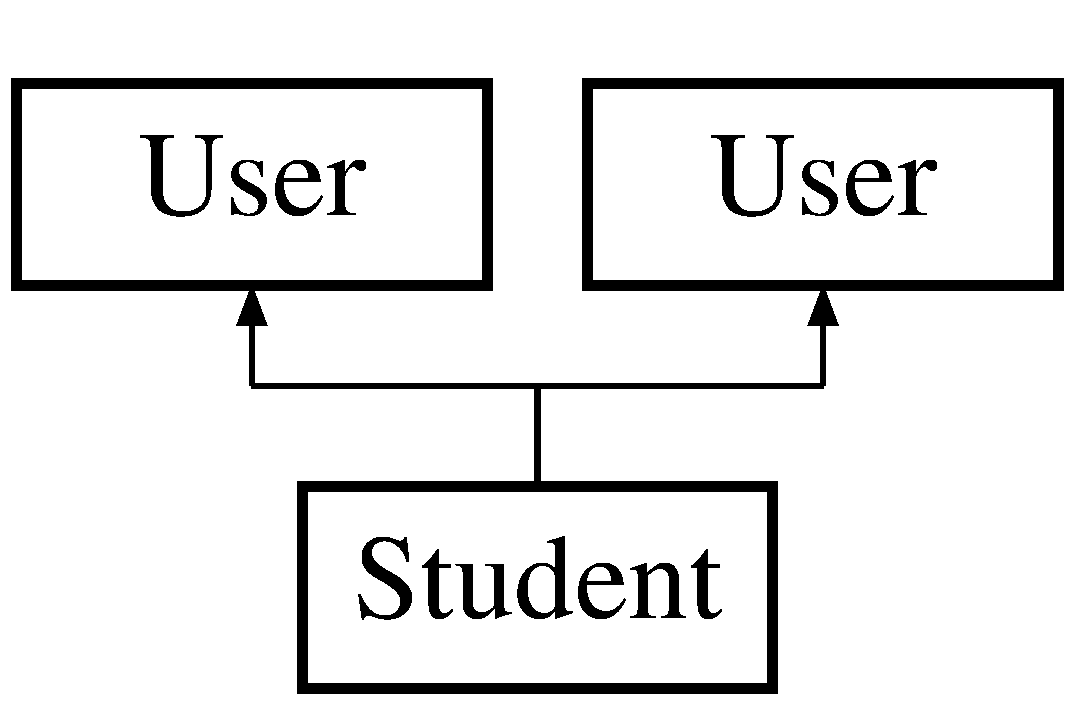
\includegraphics[height=2.000000cm]{class_student}
\end{center}
\end{figure}
\subsection*{Public Member Functions}
\begin{DoxyCompactItemize}
\item 
void \hyperlink{class_student_a11dc036cf5e771abf9ff855952a32f4a}{view\+Student} (int id)
\item 
void \hyperlink{class_student_a466ca7dba4ff1ec96455157de6e49ebf}{restart\+Quiz} ()
\item 
void \hyperlink{class_student_a11dc036cf5e771abf9ff855952a32f4a}{view\+Student} (int id)
\item 
void \hyperlink{class_student_a466ca7dba4ff1ec96455157de6e49ebf}{restart\+Quiz} ()
\end{DoxyCompactItemize}


\subsection{Detailed Description}
\hyperlink{class_student}{Student} class inherited from \hyperlink{class_user}{User} class 

\subsection{Member Function Documentation}
\hypertarget{class_student_a466ca7dba4ff1ec96455157de6e49ebf}{}\index{Student@{Student}!restart\+Quiz@{restart\+Quiz}}
\index{restart\+Quiz@{restart\+Quiz}!Student@{Student}}
\subsubsection[{restart\+Quiz()}]{\setlength{\rightskip}{0pt plus 5cm}void Student\+::restart\+Quiz (
\begin{DoxyParamCaption}
{}
\end{DoxyParamCaption}
)}\label{class_student_a466ca7dba4ff1ec96455157de6e49ebf}
function to restart quiz \hypertarget{class_student_a466ca7dba4ff1ec96455157de6e49ebf}{}\index{Student@{Student}!restart\+Quiz@{restart\+Quiz}}
\index{restart\+Quiz@{restart\+Quiz}!Student@{Student}}
\subsubsection[{restart\+Quiz()}]{\setlength{\rightskip}{0pt plus 5cm}void Student\+::restart\+Quiz (
\begin{DoxyParamCaption}
{}
\end{DoxyParamCaption}
)}\label{class_student_a466ca7dba4ff1ec96455157de6e49ebf}
function to restart quiz \hypertarget{class_student_a11dc036cf5e771abf9ff855952a32f4a}{}\index{Student@{Student}!view\+Student@{view\+Student}}
\index{view\+Student@{view\+Student}!Student@{Student}}
\subsubsection[{view\+Student(int id)}]{\setlength{\rightskip}{0pt plus 5cm}void Student\+::view\+Student (
\begin{DoxyParamCaption}
\item[{int}]{id}
\end{DoxyParamCaption}
)}\label{class_student_a11dc036cf5e771abf9ff855952a32f4a}
function to retrieve and display student profile \hypertarget{class_student_a11dc036cf5e771abf9ff855952a32f4a}{}\index{Student@{Student}!view\+Student@{view\+Student}}
\index{view\+Student@{view\+Student}!Student@{Student}}
\subsubsection[{view\+Student(int id)}]{\setlength{\rightskip}{0pt plus 5cm}void Student\+::view\+Student (
\begin{DoxyParamCaption}
\item[{int}]{id}
\end{DoxyParamCaption}
)}\label{class_student_a11dc036cf5e771abf9ff855952a32f4a}
function to retrieve and display student profile 

The documentation for this class was generated from the following files\+:\begin{DoxyCompactItemize}
\item 
main.\+cpp\item 
quiz.\+h\end{DoxyCompactItemize}

\hypertarget{class_user}{}\section{User Class Reference}
\label{class_user}\index{User@{User}}
Inheritance diagram for User\+:\begin{figure}[H]
\begin{center}
\leavevmode
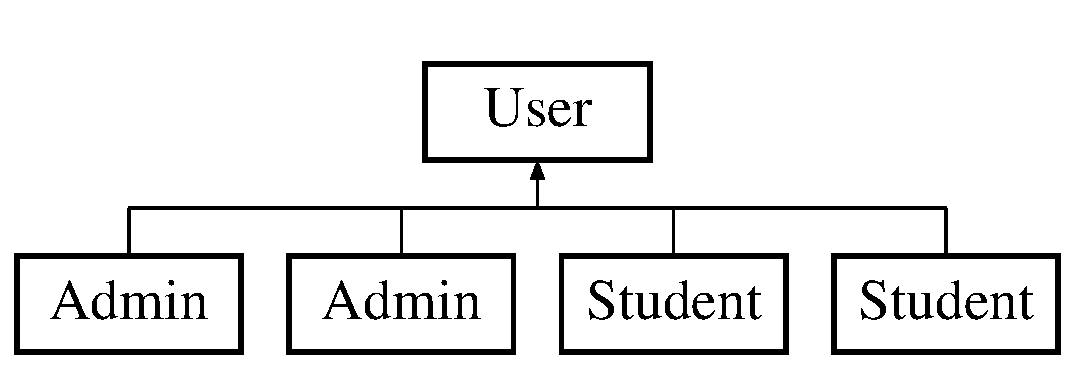
\includegraphics[height=2.000000cm]{class_user}
\end{center}
\end{figure}
\subsection*{Public Member Functions}
\begin{DoxyCompactItemize}
\item 
void \hyperlink{class_user_a7413d6e3ca3a5157beab559812a25a14}{login} (string)
\item 
void \hyperlink{class_user_a64a7433869a4ad67cf381a6d71b2f2d8}{answer} (int)
\end{DoxyCompactItemize}
\subsection*{Public Attributes}
\begin{DoxyCompactItemize}
\item 
string \hyperlink{class_user_a643f85779a4693855c171c396f49e515}{name}
\item 
int \hyperlink{class_user_aa7e6e39b43020bbe9c3a196b3689b0f7}{id}
\end{DoxyCompactItemize}


\subsection{Detailed Description}
Base class 

\subsection{Member Function Documentation}
\hypertarget{class_user_a64a7433869a4ad67cf381a6d71b2f2d8}{}\index{User@{User}!answer@{answer}}
\index{answer@{answer}!User@{User}}
\subsubsection[{answer(int)}]{\setlength{\rightskip}{0pt plus 5cm}void User\+::answer (
\begin{DoxyParamCaption}
\item[{int}]{}
\end{DoxyParamCaption}
)}\label{class_user_a64a7433869a4ad67cf381a6d71b2f2d8}
function to send an answer \hypertarget{class_user_a7413d6e3ca3a5157beab559812a25a14}{}\index{User@{User}!login@{login}}
\index{login@{login}!User@{User}}
\subsubsection[{login(string)}]{\setlength{\rightskip}{0pt plus 5cm}void User\+::login (
\begin{DoxyParamCaption}
\item[{string}]{}
\end{DoxyParamCaption}
)}\label{class_user_a7413d6e3ca3a5157beab559812a25a14}
function to login 

\subsection{Member Data Documentation}
\hypertarget{class_user_aa7e6e39b43020bbe9c3a196b3689b0f7}{}\index{User@{User}!id@{id}}
\index{id@{id}!User@{User}}
\subsubsection[{id}]{\setlength{\rightskip}{0pt plus 5cm}int User\+::id}\label{class_user_aa7e6e39b43020bbe9c3a196b3689b0f7}
integer containing user id number \hypertarget{class_user_a643f85779a4693855c171c396f49e515}{}\index{User@{User}!name@{name}}
\index{name@{name}!User@{User}}
\subsubsection[{name}]{\setlength{\rightskip}{0pt plus 5cm}string User\+::name}\label{class_user_a643f85779a4693855c171c396f49e515}
string containing user name 

The documentation for this class was generated from the following file\+:\begin{DoxyCompactItemize}
\item 
main.\+cpp\end{DoxyCompactItemize}

%--- End generated contents ---

% Index
\backmatter
\newpage
\phantomsection
\clearemptydoublepage
\addcontentsline{toc}{chapter}{Index}
\printindex

\end{document}
